% !TEX TS-program = pdflatex
% !TEX encoding = UTF-8 Unicode

% This is a simple template for a LaTeX document using the "article" class.
% See "book", "report", "letter" for other types of document.

\documentclass[11pt]{article} % use larger type; default would be 10pt

\usepackage[utf8]{inputenc} % set input encoding (not needed with XeLaTeX)

%%% PAGE DIMENSIONS
\usepackage{geometry} % to change the page dimensions
\geometry{a4paper} % or letterpaper (US) or a5paper or....

\usepackage{graphicx} % support the \includegraphics command and options

\usepackage{amssymb}
\usepackage{amsmath}
%%% PACKAGES
\usepackage{booktabs} % for much better looking tables
\usepackage{array} % for better arrays (eg matrices) in maths
\usepackage{paralist} % very flexible & customisable lists (eg. enumerate/itemize, etc.)
\usepackage{verbatim} % adds environment for commenting out blocks of text & for better verbatim
\usepackage{subfig} % make it possible to include more than one captioned figure/table in a single float
% These packages are all incorporated in the memoir class to one degree or another...

%%% HEADERS & FOOTERS
\usepackage{fancyhdr} % This should be set AFTER setting up the page geometry
\pagestyle{fancy} % options: empty , plain , fancy
\renewcommand{\headrulewidth}{0pt} % customise the layout...
\lhead{}\chead{}\rhead{}
\lfoot{}\cfoot{\thepage}\rfoot{}

%%% SECTION TITLE APPEARANCE
\usepackage{sectsty}
\allsectionsfont{\sffamily\mdseries\upshape} % (See the fntguide.pdf for font help)
% (This matches ConTeXt defaults)

%%% ToC (table of contents) APPEARANCE
\usepackage[nottoc,notlof,notlot]{tocbibind} % Put the bibliography in the ToC
\usepackage[titles,subfigure]{tocloft} % Alter the style of the Table of Contents
\renewcommand{\cftsecfont}{\rmfamily\mdseries\upshape}
\renewcommand{\cftsecpagefont}{\rmfamily\mdseries\upshape} % No bold!

\usepackage{amsmath}
\usepackage{graphicx}
\graphicspath{ {./pings/} }
\DeclareMathOperator*{\argmax}{arg\,max}
\DeclareMathOperator*{\argmin}{arg\,min}

\newcount\colveccount
\newcommand*\colvec[1]{
        \global\colveccount#1
        \begin{pmatrix}
        \colvecnext
}
\def\colvecnext#1{
        #1
        \global\advance\colveccount-1
        \ifnum\colveccount>0
                \\
                \expandafter\colvecnext
        \else
                \end{pmatrix}
        \fi
}

%%% END Article customizations

%%% The "real" document content comes below...

\title{Micro HW1}
\author{Michael B. Nattinger\footnote{I worked on this assignment with my study group: Alex von Hafften, Andrew Smith, Ryan Mather, and Tyler Welch. I have also discussed problem(s) with Emily Case, Sarah Bass, Katherine Kwok, and Danny Edgel.}}

%\date{} % Activate to display a given date or no date (if empty),
         % otherwise the current date is printed 

\begin{document}
\maketitle

\section{Question 1}
The first firm to enter the market will be the firm with the lowest fixed cost, i.e. firm $1$. This firm will choose to enter when profits are nonnegative:
\begin{align*}
pq - 1 - q - q^2 &\geq 0
\end{align*}
The firm maximizes profit:
\begin{align*}
\max_{q} pq - 1 - q - q^2\\
\Rightarrow p = 1+2q\\
\Rightarrow q = \frac{p-1}{2}
\end{align*}

Our nonnegative profit condition then yields:
\begin{align*}
\frac{p^2-p}{2} - 1 -  \frac{p-1}{2} - \left(  \frac{p-1}{2} \right)^2 &\geq 0\\
p^2 - 2p - 1 - \frac{p^2 - 2p +1}{2} \geq 0\\
p^2 - 2p -3 \geq 0\\
(p-3)(p+1) \geq 0
\end{align*}
The $p^*$ which is the minimum price to have production is the positive price which satisfies the above expression with equality. Therefore, $p^* = 3$.

\section{Question 2}
\subsection{Part A}
Given a tax level $\tau$, a firm will choose quantity to produce $q$ which maximies profits, and will enter the market if their profits are nonnegative.
\begin{align*}
\max_{x} (1-\tau)2\theta x- x^2 -1\\
\Rightarrow (1-\tau)2\theta = 2x\\
\Rightarrow x = (1-\tau)\theta.
\end{align*}
The firms enter if their profits are nonnegative:
\begin{align*}
(1-\tau)2\theta x- x^2 -1 \geq 0\\ 
(1-\tau)^22\theta^2 - (1-\tau)^2\theta^2 -1 \geq 0\\ 
\theta \geq \frac{1}{1-\tau}
\end{align*}

The aggregate supply of the firms is the integral across their distribution. Note that we are provided with a functional form for the mass of firms with ideas above a value of theta. We can convert this to a density by taking the negative of the derivative of this function: $f(\theta) = \beta \theta^{-\beta - 1}$. Then, our supply is the following:
\begin{align*}
Q_s(\tau) &= \int_{\frac{1}{1-\tau}}^{\infty}2(1-\tau)\theta^2 f(\theta)d\theta\\
&=  \int_{\frac{1}{1-\tau}}^{\infty}2(1-\tau)\theta^2\beta \theta^{-\beta - 1}d\theta \\
&= \frac{1(1-\tau) \beta}{2-\beta}[\theta^{2-\beta}]_{\frac{1}{1-\tau}}^{\infty}\\
&= \frac{2\beta(1-\tau)^{\beta - 1}}{\beta - 2}
\end{align*}
\subsection{Part B}
When Apple raises its tax rate, the cutoff moves up (i.e. fewer firms are developers). Furthermore, the amount of code each producer produces falls.
\subsection{Part C}
Apple maximizes their revenue:
\begin{align*}
\max_{\tau} \tau  \frac{2\beta(1-\tau)^{\beta - 1}}{\beta - 2}\\
\Rightarrow \frac{2\beta(1-\tau^*)^{\beta - 1}}{\beta - 2} &= \tau^{*}\frac{2\beta(1-\tau^*)^{\beta - 2}}{\beta - 2}(\beta - 1)\\
\Rightarrow \tau^{*} &= \frac{1}{\beta}.
\end{align*}
\subsection{Part D}
If $\beta$ rises then the firms become more concentrated at lower levels of ideas. Fewer firms produce, and total production falls.
\section{Question 3}
Our two inverse demand curves satisfy $P_{i}(Q) = a_i - b_i Q$ for $i \in \{ \text{3C}, \text{FB} \}$.

Ben and Jerry maximize profits:
\begin{align*}
\max_{Q_{i}} a_i Q_i - b_i Q_i^2 - M Q_i\\
\Rightarrow a_i -2 b_i Q_i - M = 0\\
\Rightarrow Q_i = \frac{a_i - M}{2 b_i}\\
\Rightarrow P_i = \frac{a_i + M}{2}
\end{align*}
Therefore, Fruit Bowl will be set to the higher price as it has the higher intercept.
\section{Question 4}
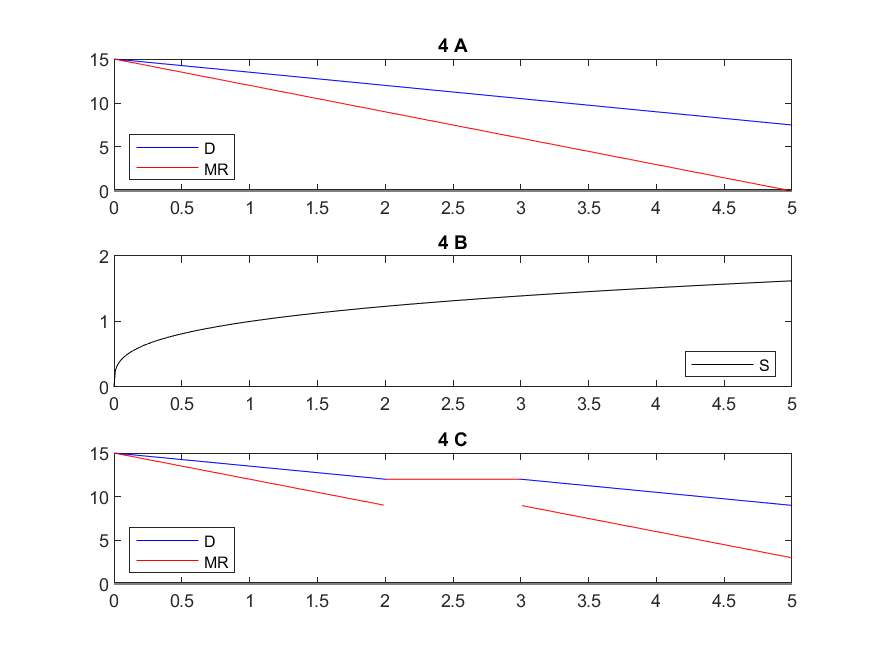
\includegraphics{q4}
\section{Question 5}
For the initial part of this question, we have that $P_i(Q_i) = a_i - Q_i$
\begin{align*}
\max_{Q_{i}} a_i Q_i -  Q_i^2 - Q_i\\
\Rightarrow a_i -2  Q_i - 1 = 0\\
\Rightarrow Q_i = \frac{a_i - 1}{2 }\\
\Rightarrow P_i = \frac{a_i + 1}{2}
\end{align*}

This implies that $P_1 = 2, P_2 = 3$. The store can make this happen by offering the higher price online and the lower price in person. Type 1 people will come in to the store and get the lower price, while Type 2 people will order online and be charged the higher price.

When the marginal cost varies by total quantity sold, the two problems become linked by the cost function and, therefore, we have a single optimization to solve.
\begin{align*}
MR=MC,\\
3 - 2q_1 = q_1 + q_2,\\
5 - 2q_2 = q_1 + q_2.
\end{align*}

We solve this system: $q_1 = 1/2,q_2 = 3/2, p_1 = 5/2, p_2 = 7/2$.
\end{document}
